\documentclass[12pt, a4paper]{article} 
\usepackage{eurosym}  
\usepackage[margin = 1.2in]{geometry}
\usepackage[french]{babel}
\usepackage[utf8x]{inputenc}
\usepackage{graphicx}
\usepackage[T1]{fontenc}
\usepackage{fancyhdr}
\pagestyle{fancy}
\setlength{\headheight}{15pt}
\fancyhead[L]{SharpBoy}
\fancyhead[R]{EPITA}
\fancyhead[C]{S\_Society}
\renewcommand{\footrulewidth}{1pt} 
\fancyfoot[L]{Cahier des charges}
\fancyfoot[R]{2016-2017}
\fancyfoot[C]{\thepage}
\title{\Huge \bf SharpBoy}
\author{\LARGE \bf S\_Society }



\begin{document}


\maketitle


\bigskip
\large Gabriel DUQUE: duque\_g

\bigskip
\large Antoine MARTIN: ma\_9

\bigskip
\large Martin MEUNIER : meunie\_o

\bigskip
\large Ilyes NOUMRI : noumri\_i

\bigskip
\large {\textbf{Projet S2\#}}

\bigskip 
\bigskip
\bigskip



\begin{center}

\includegraphics[width= 12cm]{logo-epita-hd.png} 
\end{center}


\pagebreak

\small

\tableofcontents 

\pagebreak

\large
\section{Introduction}
Pour ce premier projet à EPITA, les membres de S\_Society ont souhaité réaliser un projet algorithmiquement complexe mais toutefois ludique. Étant donné que le sujet est libre, nous avons décidé de nous lancer dans l’implémentation d’un émulateur de GameBoy en F\#.

\medskip

C’est pour nous une opportunité intéressante de pouvoir faire ce sujet car c’est une façon d’apprendre les subtilités de l’émulation. Nous découvrirons aussi le fonctionnement de l’une de nos consoles favorites. Chacun des membres du groupe ayant déjà joué à cette console, c’est donc avec un enthousiasme général que nous allons tout mettre en œuvre pour proposer un logiciel à la fois fonctionnel et facile d’utilisation, pour permettre à tous les utilisateurs nostalgiques de se remémorer de vieux souvenirs.

\medskip

À travers ce cahier des charges, nous allons présenter ce que nous souhaitons réaliser dans les moindres détails, pourquoi nous nous sommes tournés vers un émulateur et bien sûr pourquoi nous comptons le réaliser en F\#. De plus, ce cahier des charges présentera aussi l'organisation de notre groupe et la répartition des tâches que nous avons jugée juste.

\medskip

Les émulateurs représentent aujourd'hui la volonté de la communauté des joueurs de ne pas vouloir laisser mourir les vielles consoles. C'est dans cette optique de travail, progression, mais aussi de plaisir que nous vous présentons aujourd'hui le cahier des charges ci-après.
\bigskip
\bigskip
\bigskip
\begin{center}

\includegraphics[width= 10cm]{sharpboylogo.png}
\end{center}
\bigskip
\pagebreak

\section{Présentation}
\subsection{Présentation du projet}
\bigskip
La SharpBoy prendrait la forme d'un émulateur de GameBoy classique pour PC. Lors de l'exécution du fichier binaire l'utilisation se verrait dirigé vers le menu principal de la SharpBoy. 
\medskip

En premier lieu, ce menu permettra de charger une ROM de GameBoy. En cas de ROM non compatible, l'émulateur redirigera l'utilisateur vers le menu principal avec un message d'erreur lui indiquant qu'elle ne l'est pas. La Sharp Boy permettra aussi à l'utilisateur d'avoir accès à ses sauvegardes de jeu pour pouvoir les exporter vers un autre PC, voire un autre émulateur, mais aussi de charger une sauvegarde d'un jeu. Ces sauvegardes pourraient être réalisées de manière classique au cours du jeu ou bien à tout moment du jeu grâce à l'émulateur sans perturber le bon fonctionnement du jeu. 
\medskip

En outre, certaines fonctionnalités classiques de tout logiciel de jeu ou multimédia seront implémentées: pause, lecture, muet... Par ailleurs, la SharpBoy se verra implémenter un menu de configuration permettant à l'utilisateur de modifier les touches du clavier utilisées pour jouer.
\medskip

Bien évidemment, la Sharp Boy permettra d'exécuter la majorité des ROMs de GameBoy et d'y jouer de manière fluide.
\medskip

Au fur et à mesure du projet, certaines fonctionnalités pourraient venir se greffer à la Sharp Boy. Pour faciliter la transition vers les nouvelles versions, nous allons implémenter un updater indiquant à l'utilisateur si sa Sharp Boy est à jour. Sinon, elle désinstallera la version présente sur le PC et installera la nouvelle version en conservant la configuration personnelle de l'utilisateur.

\pagebreak
\subsection{La GameBoy}

\subsubsection{Histoire}

Nintendo est une des marques japonaises ayant le plus de succès au monde. Initialement, elle fabriquait des cartes a jouer avant de se tourner vers le marché naissant du jeu vidéo. Elle figure aujourd'hui parmi les firmes de jeu vidéo les plus réputées au monde avec son chiffre d'affaires de 660 millions d'euros en 2015.
\medskip

Nintendo est à l'origine des plus grandes séries de jeu vidéo, notamment les jeux dérivant de l'univers de Mario. Après la NES, console de salon devenue mythique (orginellement appelée Famicom), Nintendo développe la première console portable à cartouches interchangeables: la GameBoy. \\
De la même puissance qu'une NES, la petite console portable possède une écran de basse qualité leur permettant de la vendre à un prix raisonnable pour une telle technologie à l'époque.
\medskip

C'est évidemment un énorme succès qui assurera à la firme une place majeure dans l'industrie du jeu vidéo pour les années à venir.


\begin{center}
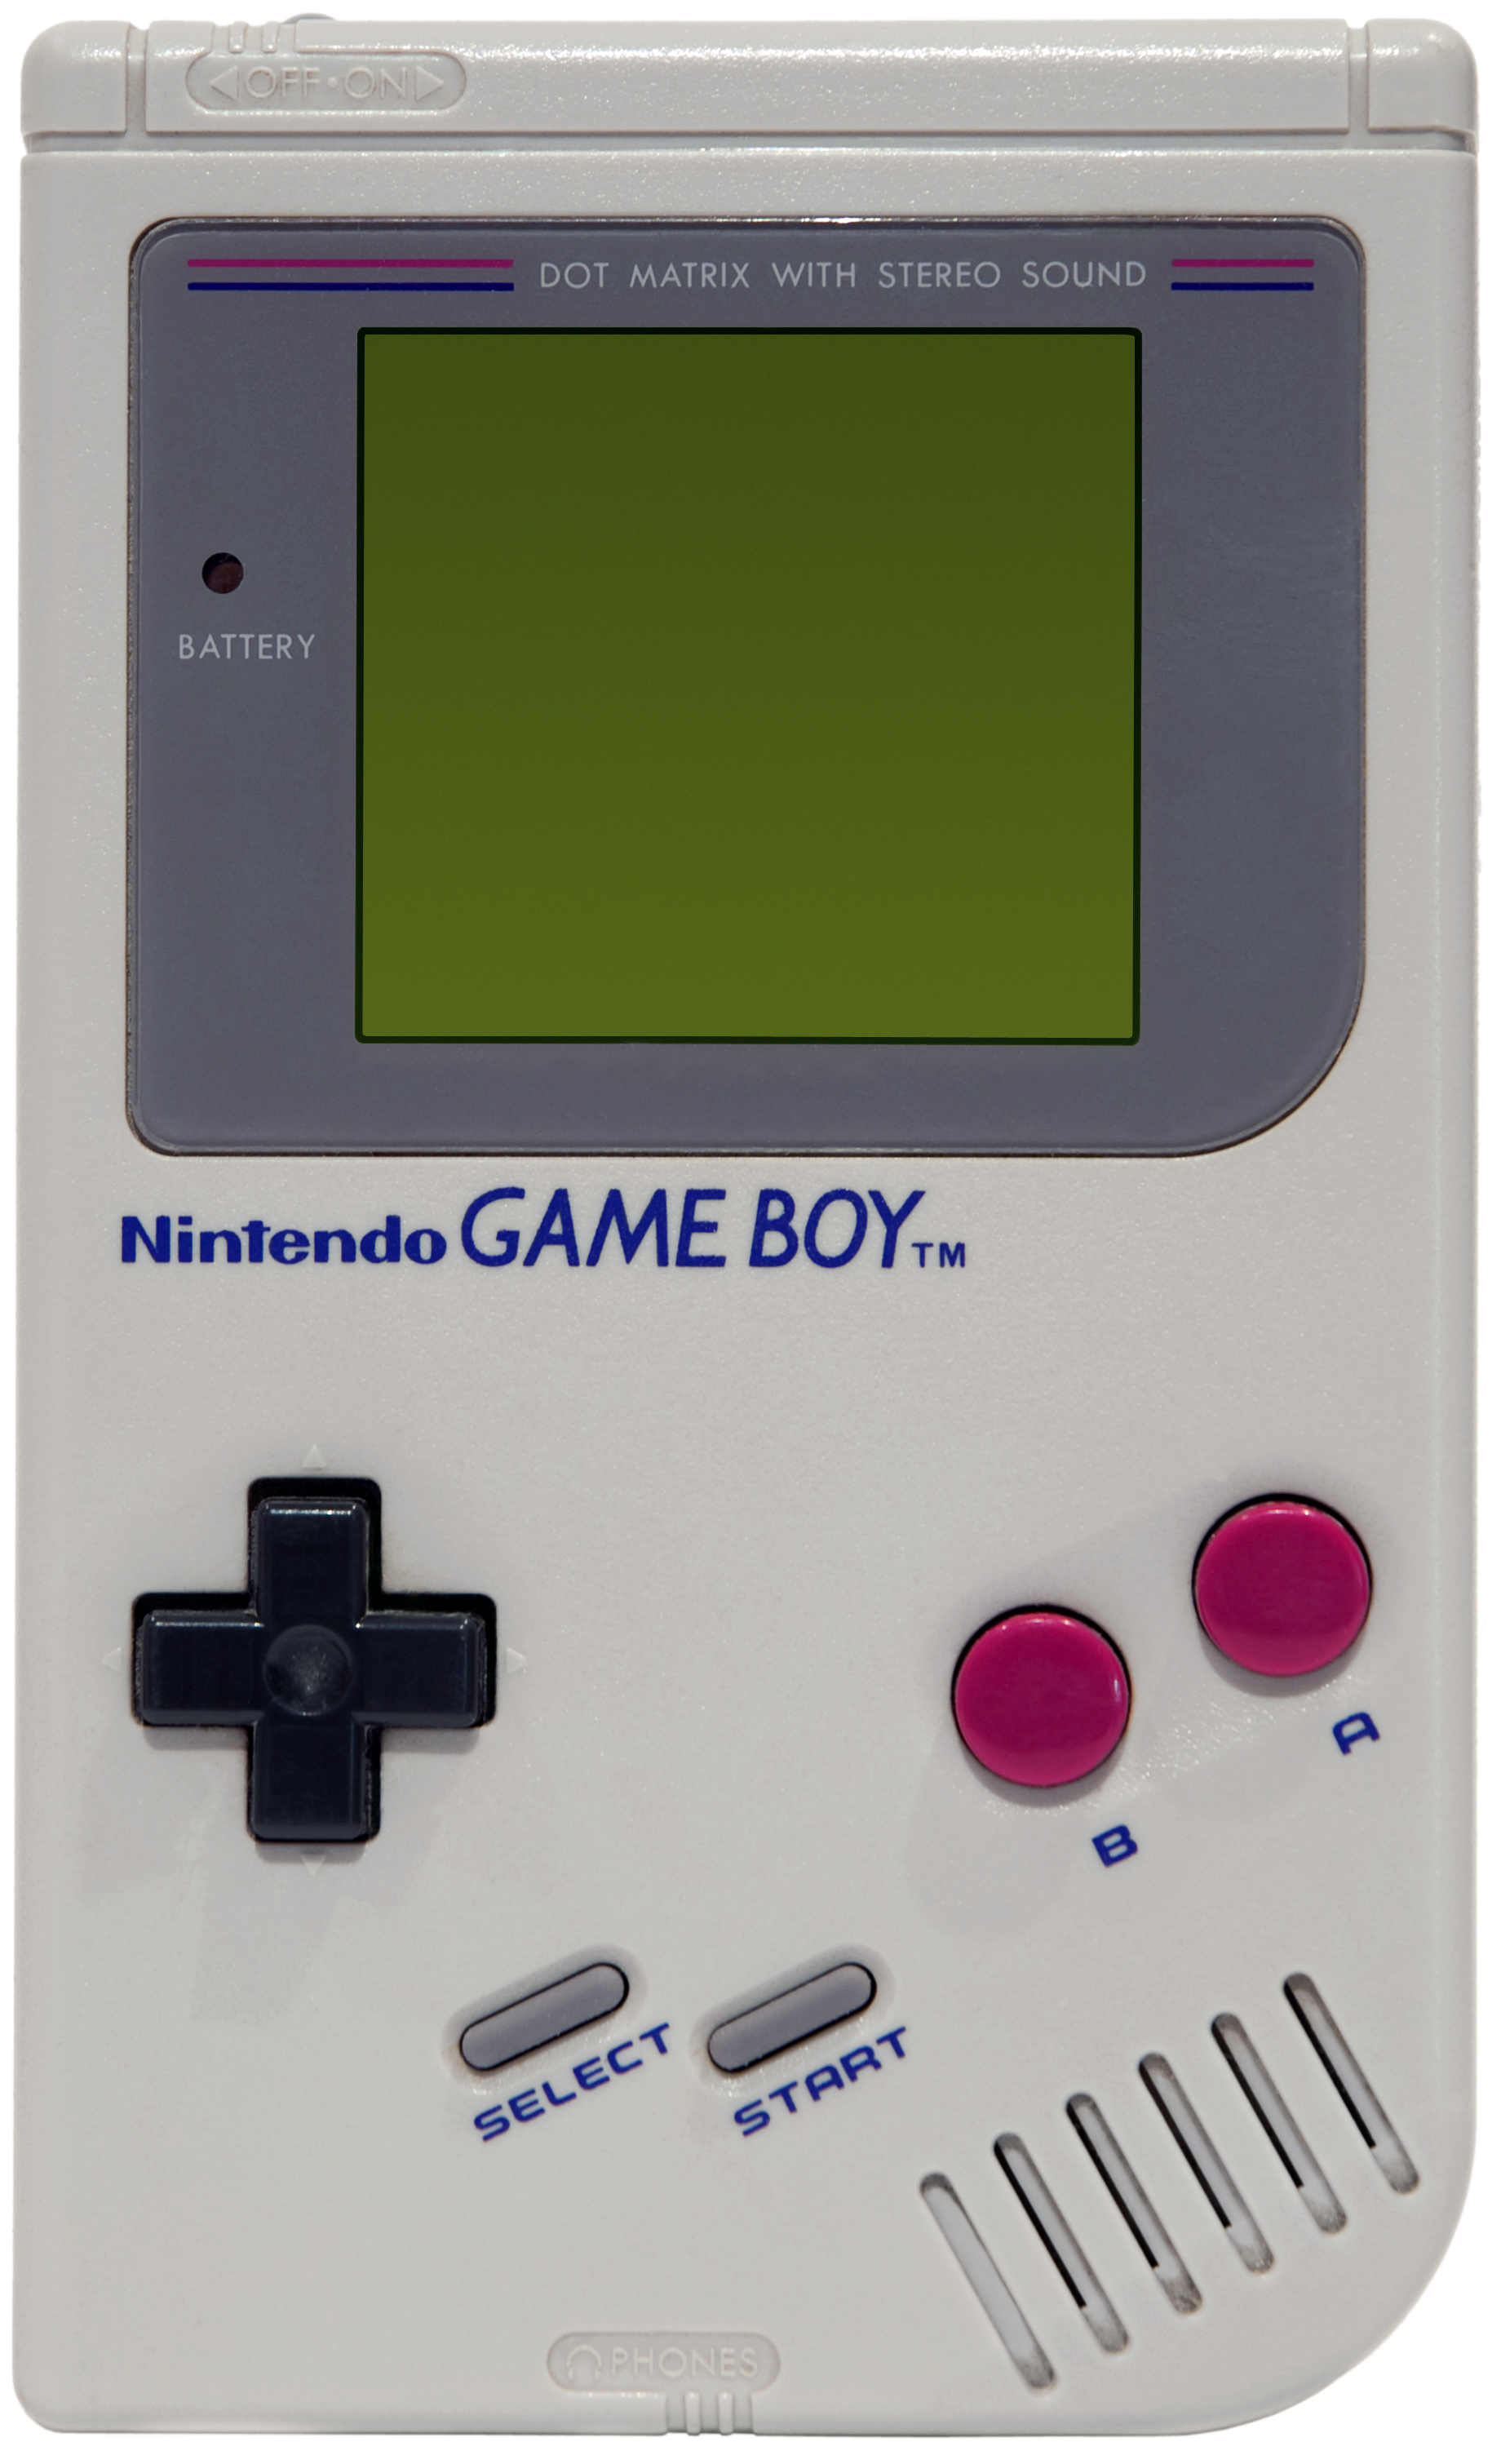
\includegraphics[width= 7cm]{nintendo-gameboy.jpg}
\end{center}

\pagebreak

\subsubsection{Description Technique}

\begin{center}
\begin{tabular}{|l|c|}
\hline
\bf Composant & \bf Caractéristiques \\
\hline 
Processeur & Sharp Z80 Custom : \\
principal & LR35902 mono-coeur cadencé a 4.19 MHz \\
\hline
RAM & 8kb (extensible a 32 kb) \\
\hline
Video RAM & 8kb\\
\hline
ROM & Cartouche de 256,512 kb et 1, 2,4 et 8 Mb\\
\hline
Son & Stéréo  \\
\hline 
Affichage & Ecran LCD 2.6pouces 160*144 Pixels  \\
\hline
Palette de couleurs & 2-bit (avec 4 nuances de gris) \\
\hline
Puissance & 6V, 0,7 W\\
\hline
Dimensions & 90*148*32 \\
\hline
\end{tabular}
\end{center}
\bigskip
\bigskip
\bigskip

\begin{center}
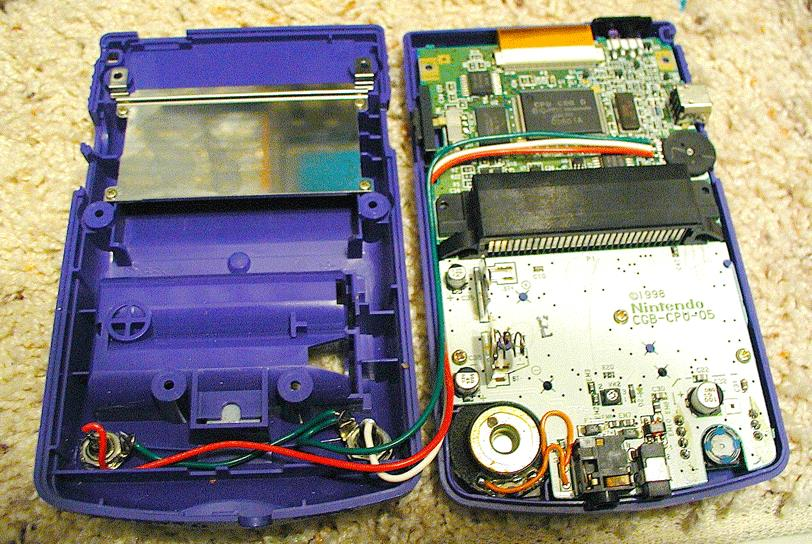
\includegraphics[width= 13.5cm]{gtainside.JPG}
\end{center}


\pagebreak



\subsection{Présentation du groupe}
\bigskip
Nous nous connaissons depuis la S1\# et nous nous sommes naturellement mis ensemble grâce à notre bonne entente et notre volonté de réaliser un projet intéressant et complet. Nous nous sommes rapprochés du fait de notre passion commune pour Linux. 
\medskip

Gabriel et Antoine étaient également dans le même amphi en médecine avant de rejoindre l'EPITA, et se sont retrouvés aux oraux d'admission pour la classe de sharp.
\medskip

Gabriel: "Salut, je crois qu'on est dans la même classe pour cette année, je vois que tu joues à Pokémon sur ton téléphone mais je ne reconnais pas de quelle version il s'agit ..." 
Ilyes: "C'est Pokémon: Glazed un hack-rom de la version émeraude !"
... Et s'en est suivi une amitié nouvelle qui persiste aujourd'hui. Nous sommes tous des fans d'émulateurs (notamment ceux de GameBoy) et il semble donc justifié que nous nous attelions au présent projet.
\medskip

Martin nous a rejoint lors de la semaine Recherche et Innovation en début de S2\#, car nous partagions une vision commune de projet innovant.
\medskip

La programmation nous passionnant tous, c’est avec joie que nous nous attaquons à ce projet d’émulateur, ayant conscience qu’il requiert des connaissances que nous allons devoir acquérir en parallèle des enseignements de l'école.
\medskip

\pagebreak

\subsection{Présentation des membres}
\bigskip
\textbf{Gabriel “nek0chan” DUQUE (duque\_g):} 
\medskip

Faisant partie de ceux nés dans les années 90’, la GameBoy a bercé mon enfance au fil de nombreux jeux devenus classiques: la série Mario bros, Pokémon, Metroid, Castlevania… En grandissant, mon intérêt pour les nouveaux jeux vidéos s’est amenuisé, laissant place à un rythme de jeu occasionnel sur de vieux jeux grâce à la propagation et la généralisation des émulateurs sur mobile.
\medskip

En outre, je suis très intéressé par la compréhension plus profonde du fonctionnement d’un ordinateur et notamment du  processeur. Je suis un passionné de Linux et de cybersécurité. Je suis donc ravi de pouvoir approfondir mes connaissances des concepts de base de l’informatique et du fonctionnement des machines.
\medskip

Enfin, l’expérience accumulée me permettra de mieux appréhender mon travail, en autonomie et en groupe, d’apprendre la rigueur nécessaire au métier d’ingénieur.
\bigskip
\bigskip

\textbf{Antoine “alarsyo” MARTIN (ma\_9) :} 
\medskip  

Comme mes camarades j’ai grandi avec la GameBoy et ses jeux, c’est donc très intéressé que je me suis lancé sur ce projet, qui promet un grand moment de nostalgie quand notre première ROM Tetris bootera correctement. 
\medskip

Un émulateur GameBoy m’a tenu compagnie lors de longs après-midis en amphi de biochimie, avant de rejoindre l’EPITA. Je m'étais toujours demandé comment ce genre de technologie fonctionnait, c’est donc le moment d’en découvrir plus !
\medskip

Hormis l'intérêt pour la plateforme elle même, je pense que travailler sur de l’émulation peut être extrêmement formateur et m’apporter pas mal de connaissances supplémentaires. Le F\# est également un langage qui m'intéresse, ayant beaucoup aimé la manière de fonctionner du Caml, et les principes de la programmation fonctionnelle que l’on a pu aborder en cours.
\bigskip

\pagebreak

\textbf{Ilyes  NOUMRI (noumri\_i) :}
\medskip

Depuis que je suis petit, je joue sur PC à différents émulateurs et notamment des émulateurs GameBoy. C’est pourquoi, l’idée de développer un émulateur GameBoy m’a vraiment emballé !
\medskip

Je suis aussi intéressé par le fonctionnement des processeurs et des ordinateurs en général. J’ai rencontré Antoine et Gabriel l’année dernière en classe de sharp et ayant de nombreux points communs on est devenu rapidement amis. 
\medskip

J’ai connu Martin de mon année de S1 car il était dans ma classe et il a vite rejoint l’équipe . Le projet pourrait nous apporter pleins de connaissances sur le fonctionnement des CPU qui pourraient nous être utile personnellement et pour le reste de nos études.
\bigskip
\bigskip
\bigskip

\textbf{Martin “Mecha” MEUNIER (meunie\_o) :} 
\medskip 

Ayant rejoint EPITA en 2015 et ayant refais mon S1, je repars avec de meilleures bases dans toutes les matières.
\medskip

Nous nous sommes retrouvés avec mes amis pour ce projet s’annonçant palpitant ! J’ai toujours aimé les anciennes consoles car nous avons tous grandis avec quelques une comme la Gameboy et nous allons maintenant coder notre premier émulateur. C’est une fierté pour moi de faire ce projet d’émulateur et je suis, comme mes amis, super motivé pour le mener à bout.
\medskip

Le fonctionnement des CPU est très intéressant et nous avons tous voulus y prêter attention. J’espère que ce projet m’apportera d’énormes connaissances pour la suite de ma scolarité à EPITA. De plus, le fait de faire du F\# m'intéresse vraiment et cela donne l’impression d’un vrai challenge de projet. J’espère que ce projet vous plaira autant qu’il nous a plu.
\bigskip
\bigskip


\pagebreak

\section{Objet de l'étude}

Notre projet possède différents intérêts pour notre groupe mais aussi individuellement. En effet, la création d'un émulateur de A à Z nous permet de comprendre complètement son fonctionnement. De plus, grâce à notre projet, chacun peut s'améliorer en programmation. Le projet étant en F\#, c'est essentiellement ce langage que nous maîtriserons à la fin du projet. Ce langage étant de plus un langage très majoritairement influencé par le C\# et le OCaml, langages que nous étudions, il nous permettra de comprendre, à travers l'analyse de sa syntaxe et la comparaison aux deux langages connus, certains concepts algorithmiques  dénués de l'étiquette des langages et ainsi développer notre compréhension des outils que nous manipulons. 
\medskip

Ensuite, ce travail de groupe est très intéressant pour optimiser le travail de chacun avec les autres et travailler efficacement les uns avec les autres. Plusieurs buts sont associés à ce projet bien que le but principal soit de présenter un émulateur qui fonctionne. 
En premier lieu, en guise d'introduction dans le monde de l'émulation, nous allons réaliser un émulateur de Chip-8 avant de monter progressivement en difficulté pour finir par un émulateur de GameBoy de bonne qualité et permettant un jeu fluide. 
\medskip

Finalement,le fait de réaliser un projet dans un cadre tel que celui-ci qui est quasi professionnel avec des limites temporelles et des dossiers à rendre avec des caractéristiques à respecter pour le rendu final et le cahier de charges va nous donner une idée du déroulement de la phase de développement dans une vraie entreprise.

\pagebreak
\section{État de l'art}
L'émulation dans le domaine du jeu vidéo est un phénomène apparu dans les années 90’ . Les premiers émulateurs étaient principalement deux machines émulant le fonctionnement de consoles Nintendo des années 80’. 
\medskip

Bien que l'évolution des consoles est rapide, les débuts de l'émulation ont été un vrai défi technique. En effet, les entreprises de consoles ne dévoilent pas les détails techniques des consoles, contraignant les jeunes programmeurs à comprendre petit à petit d’eux mêmes le fonctionnement des machines. \\
De ce fait, les premiers émulateurs ne comportaient pas la totalité des fonctionnalités des consoles, ou bien présentaient de nombreux bugs...

\medskip

De nos jours, les émulateurs sont assez communs et ils existent pour la majorité des consoles.Par la suite, les avancées d'internet permettant un partage plus rapide des connaissances et des concepts informatiques a permis l'expansion massive des émulateurs pour PC et téléphones mobiles. La console de jeu la plus fréquemment émulée reste la GameBoy Advance. 

\medskip

L’expansion des émulateurs ne cesse de standardiser leurs usages avec de nombreuses fonctions se trouvant dans la grande majorité d’entre eux, permettant parfois même une progression par rapport aux consoles de base. Ces améliorations ont été permises entre autres par la progression de la puissance de calcul des machines notamment les ordinateurs et les téléphones.  Par exemple, la majorité des émulateurs de GameBoy peuvent accélérer ou ralentir le jeu à la guise de l’utilisateur, prendre des captures d’écran, enregistrer le gameplay ou même sauvegarder la partie dans des endroits du jeu où ce n’était pas prévu dans le jeu originel. Associés à la mobilité absolue des émulateurs sur mobile, la facilité avec laquelle les jeux sont téléchargeables et le peu de mémoire de stockage qu’ils occupent, les émulateurs permettent aujourd’hui à des nombreux nostalgiques de retrouver dans le métro leurs jeux favoris.

L'émulateur de GameBoy occupant la place la plus importante est sans aucun doute VisualBoy Advance, gérant de la GameBoy à la GameBoy Advance et comportant toutes les fonctionnalités nécessaires.


\pagebreak
\section{Travail à réaliser}

\subsection{Tâches}

\bigskip



\subsubsection{Interface}
Le menu permettra de régler l'émulateur selon les préférences de l'utilisateur notamment l'assignation des touches et le chargement des ROM ; il permettra également de prendre des captures d'écran ou de mettre en pause l'émulateur (fonctionnalité impossible sur une vraie console).

\subsubsection{Site web}
Construction du site web pour notre projet avec un lien de téléchargement du projet ainsi que des informations sur le groupe, la nature du projet 

\subsubsection{Vidéo}
Fonctions d'affichage du jeu sur l'émulateur.

\subsubsection{CPU}
Coeur de l’émulateur, permet de traduire les instructions et effectuer les tâches correspondantes.

\subsubsection{Mémoire}
Allocation mémoire pour l’émulateur, pour le bon fonctionnement du logiciel.

\subsubsection{Audio}
Gestion de la sortie sonore du jeu et de la synchronisation des évènements et du lancement des sons correspondants

\subsubsection{Réseau}
Updater permettant à l'utilisateur d'accéder à la dernière version du logiciel

\pagebreak

\subsection{Répartition des tâches}

\bigskip
\bigskip


\begin{center}
\begin{tabular}{|l|c|c|c|c|}
\hline
\bf Tâches                & \bf Gabriel   & \bf Antoine   & \bf Martin    & \bf Ilyes\\
\hline 
Menus/Options       &      x       &               &         x     &       \\
\hline 
Site web            &               &         x     &               &     x  \\
\hline 
Vidéo               &          x    &               &       x       &       \\
\hline 
CPU                 & x             & x             &               &       \\
\hline 
Mémoire             &               & x             &               &  x \\
\hline
Audio               &               &               & x             & x \\
\hline
Marketing           & x             &               &               & x \\
\hline
Réseau              &               &               & x             & x \\ 
\hline
\end{tabular}
\end{center}
\bigskip
\bigskip
\bigskip

\section{Planning}
\bigskip
\bigskip

\begin{center}
\begin{tabular}{|l|c|c|c|}
\hline
\bf Tâches          & \bf Soutenance 1      & \bf Soutenance 2      & \bf Soutenance 3  \\
\hline 
Menus/Options       &      0\%                 &         0\%              &     100\%    \\
\hline 
Site web            &        66\%             &        100\%          &         100\%       \\
\hline 
Vidéo               &       33\%               &         66\%            &     100\%  \\
\hline 
CPU                 & 33\%                     &  66\%                   &   100\%    \\
\hline 
Mémoire             & 66\%                   & 100\%                   & 100\%  \\
\hline
Audio               &    0\%                   & 33\%                     & 100\%  \\
\hline
Réseau              & 0\%                   & 25\%                     & 100\%  \\

\hline
\end{tabular}

\end{center}




\pagebreak



\section{Ressources}

\bigskip
\subsection{Github}
Nous utiliserons le site web Github pour que l'on puisse travailler et collaborer efficacement sur le projet. 
\medskip

Il servira aussi pour l'hébergement du site, grâce à Github Pages, et hébergera les différentes mises à jour.


\bigskip
\subsection{Visual Studio, Monodevelop}
Ayant déjà utilisé ces IDEs pour réaliser les TPs du S1\# l'ensemble du groupe est à l'aise avec ces logiciels. 
\medskip

Ces IDEs ont une interface connu et permettent d'exploiter tous les aspects et les bibliothèques de F\#, ainsi que le debugger et le compilateur.

\bigskip
\subsection{ROMs de tests}
Nous utiliserons des sets de ROMs spécifiques destinés à tester toutes les fonctions de l'émulateur.
\medskip

Les ROMs de test de Blargg (http://slack.net/~ant/old/gb-tests/) ciblent les différentes fonctionnalités nécessaires à l'émulateur (instructions CPU, timing mémoire...).

\bigskip
\subsection{GameBoy Technical Documentation}
 Nous utiliserons la documentation technique de la GameBoy pour comprendre le fonctionnement de son système et de ses composants, ainsi que pour la description des 252 instructions processeur.

\pagebreak

\bigskip
\subsection{fsharp.org}
Pour la documentation concernant le F\#. En effet, ce site regroupe l'ensemble des informations nécéssaires au développement en F\# ainsi que les bibliothèques nécéssaires à notre projet.  

\bigskip
\subsection{MSDN}
Ce site contient également de nombreuses ressources pour le F\#, c'est un terrain familier puisque nous l'utilisons tous beaucoup en IP pour le C\#.
\medskip

Nous aurons aussi recours à différents forums (StackOverflow notamment) pour rassembler toutes les informations nécessaires à la réalisation de notre projet, notamment pour le réseau.

\pagebreak

\section{Aspects économiques}
\subsection{Matériel}

\bigskip

\begin{center}
\begin{tabular}{|l|c|}
\hline
\bf Entité & \bf Prix \\
\hline 
Desktop Antoine & 670€\\
\hline
Desktop Ilyes & 700€ \\
\hline
Lenovo Yoga 500 & 800€\\
\hline
ASUS RoG G751 & 1500€ \\
\hline
La chaise IKEA d'Antoine & 39€ \\
\hline 
Le bureau IKEA d'Antoine & 109€ \\
\hline
Le tapis de souris Diablo III d'Antoine & 15€\\
\hline
La souris d'Antoine & 40€ \\
\hline
\bf Coût total & \bf 3873€\\
\hline
\end{tabular}
\end{center}

\subsection{Logiciel}

\bigskip

\begin{center}
\begin{tabular}{|l|c|}
\hline
\bf Entité & \bf Prix \\
\hline 
Visual Studio & 0€ (thx MSDNAA)\\
\hline
MonoDevelop & Quelques bibliothèques\\
\hline
Chrome & Mon droit à la vie privée \\ 
\hline
Licences Windows & 0€ \\
\hline
Fedora 24 & Un boot rapide\\
\hline
Ubuntu & Dignity \\
\hline 
Glorious ArchLinux & Linus Torvalds has my soul now \\
\hline
f.lux & 0€ \\
\hline
\bf Coût total & \bf 0€\\
\hline
\end{tabular}
\end{center}



\subsection{Vivres}

\bigskip

\begin{center}
\begin{tabular}{|l|c|c|}
\hline
\bf Entité & \bf Quantité & \bf Prix \\
\hline 
Kebab & ALL OF IT & 5€ x 378\\
\hline
Pizza & Industrielle & 0€ (Sponsor) \\
\hline
Boisson énergisantes & Exponentielle & Notre humeur \\
\hline
\bf Total & \bf Beaucoup  & \bf Too damn high \\
\hline
\end{tabular}
\end{center}

\pagebreak

\section{Conclusion}
Développer un émulateur n'est pas une tâche aisée pour des personnes à priori limitées en programmation : c'est pour quoi une grande rigueur de travail quelque peu similaire à un cadre professionnel nous sera nécessaire tout au long du projet.
\medskip

Notre but est avant tout d'apprendre un maximum de cette expérience, qui non seulement nous sera bénéfique pour notre culture générale d'ingénieur en informatique mais aussi pour la suite de nos études. \\
Nous espérons que le projet final saura satisfaire notre jury, nous satisfera personnellement et qu'il nous ouvrira la porte à d'autres projets dans le domaine de l'émulation. 

\end{document}
